\documentclass[1p]{elsarticle_modified}
%\bibliographystyle{elsarticle-num}

%\usepackage[colorlinks]{hyperref}
%\usepackage{abbrmath_seonhwa} %\Abb, \Ascr, \Acal ,\Abf, \Afrak
\usepackage{amsfonts}
\usepackage{amssymb}
\usepackage{amsmath}
\usepackage{amsthm}
\usepackage{scalefnt}
\usepackage{amsbsy}
\usepackage{kotex}
\usepackage{caption}
\usepackage{subfig}
\usepackage{color}
\usepackage{graphicx}
\usepackage{xcolor} %% white, black, red, green, blue, cyan, magenta, yellow
\usepackage{float}
\usepackage{setspace}
\usepackage{hyperref}

\usepackage{tikz}
\usetikzlibrary{arrows}

\usepackage{multirow}
\usepackage{array} % fixed length table
\usepackage{hhline}

%%%%%%%%%%%%%%%%%%%%%
\makeatletter
\renewcommand*\env@matrix[1][\arraystretch]{%
	\edef\arraystretch{#1}%
	\hskip -\arraycolsep
	\let\@ifnextchar\new@ifnextchar
	\array{*\c@MaxMatrixCols c}}
\makeatother %https://tex.stackexchange.com/questions/14071/how-can-i-increase-the-line-spacing-in-a-matrix
%%%%%%%%%%%%%%%

\usepackage[normalem]{ulem}

\newcommand{\msout}[1]{\ifmmode\text{\sout{\ensuremath{#1}}}\else\sout{#1}\fi}
%SOURCE: \msout is \stkout macro in https://tex.stackexchange.com/questions/20609/strikeout-in-math-mode

\newcommand{\cancel}[1]{
	\ifmmode
	{\color{red}\msout{#1}}
	\else
	{\color{red}\sout{#1}}
	\fi
}

\newcommand{\add}[1]{
	{\color{blue}\uwave{#1}}
}

\newcommand{\replace}[2]{
	\ifmmode
	{\color{red}\msout{#1}}{\color{blue}\uwave{#2}}
	\else
	{\color{red}\sout{#1}}{\color{blue}\uwave{#2}}
	\fi
}

\newcommand{\Sol}{\mathcal{S}} %segment
\newcommand{\D}{D} %diagram
\newcommand{\A}{\mathcal{A}} %arc


%%%%%%%%%%%%%%%%%%%%%%%%%%%%%5 test

\def\sl{\operatorname{\textup{SL}}(2,\Cbb)}
\def\psl{\operatorname{\textup{PSL}}(2,\Cbb)}
\def\quan{\mkern 1mu \triangleright \mkern 1mu}

\theoremstyle{definition}
\newtheorem{thm}{Theorem}[section]
\newtheorem{prop}[thm]{Proposition}
\newtheorem{lem}[thm]{Lemma}
\newtheorem{ques}[thm]{Question}
\newtheorem{cor}[thm]{Corollary}
\newtheorem{defn}[thm]{Definition}
\newtheorem{exam}[thm]{Example}
\newtheorem{rmk}[thm]{Remark}
\newtheorem{alg}[thm]{Algorithm}

\newcommand{\I}{\sqrt{-1}}
\begin{document}

%\begin{frontmatter}
%
%\title{Boundary parabolic representations of knots up to 8 crossings}
%
%%% Group authors per affiliation:
%\author{Yunhi Cho} 
%\address{Department of Mathematics, University of Seoul, Seoul, Korea}
%\ead{yhcho@uos.ac.kr}
%
%
%\author{Seonhwa Kim} %\fnref{s_kim}}
%\address{Center for Geometry and Physics, Institute for Basic Science, Pohang, 37673, Korea}
%\ead{ryeona17@ibs.re.kr}
%
%\author{Hyuk Kim}
%\address{Department of Mathematical Sciences, Seoul National University, Seoul 08826, Korea}
%\ead{hyukkim@snu.ac.kr}
%
%\author{Seokbeom Yoon}
%\address{Department of Mathematical Sciences, Seoul National University, Seoul, 08826,  Korea}
%\ead{sbyoon15@snu.ac.kr}
%
%\begin{abstract}
%We find all boundary parabolic representation of knots up to 8 crossings.
%
%\end{abstract}
%\begin{keyword}
%    \MSC[2010] 57M25 
%\end{keyword}
%
%\end{frontmatter}

%\linenumbers
%\tableofcontents
%
\newcommand\colored[1]{\textcolor{white}{\rule[-0.35ex]{0.8em}{1.4ex}}\kern-0.8em\color{red} #1}%
%\newcommand\colored[1]{\textcolor{white}{ #1}\kern-2.17ex	\textcolor{white}{ #1}\kern-1.81ex	\textcolor{white}{ #1}\kern-2.15ex\color{red}#1	}

{\Large $\underline{12a_{1184}~(K12a_{1184})}$}

\setlength{\tabcolsep}{10pt}
\renewcommand{\arraystretch}{1.6}
\vspace{1cm}\begin{tabular}{m{100pt}>{\centering\arraybackslash}m{274pt}}
\multirow{5}{120pt}{
	\centering
	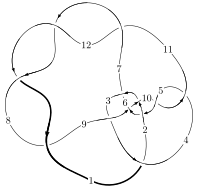
\includegraphics[width=112pt]{../../../GIT/diagram.site/Diagrams/png/1985_12a_1184.png}\\
\ \ \ A knot diagram\footnotemark}&
\allowdisplaybreaks
\textbf{Linearized knot diagam} \\
\cline{2-2}
 &
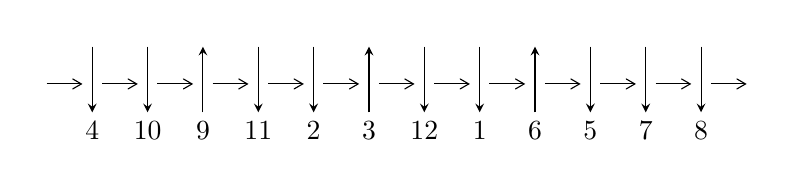
\begin{tikzpicture}[x=20pt, y=17pt]
	% nodes
	\node (C0) at (0, 0) {};
	\node (C1) at (1, 0) {};
	\node (C1U) at (1, +1) {};
	\node (C1D) at (1, -1) {4};

	\node (C2) at (2, 0) {};
	\node (C2U) at (2, +1) {};
	\node (C2D) at (2, -1) {10};

	\node (C3) at (3, 0) {};
	\node (C3U) at (3, +1) {};
	\node (C3D) at (3, -1) {9};

	\node (C4) at (4, 0) {};
	\node (C4U) at (4, +1) {};
	\node (C4D) at (4, -1) {11};

	\node (C5) at (5, 0) {};
	\node (C5U) at (5, +1) {};
	\node (C5D) at (5, -1) {2};

	\node (C6) at (6, 0) {};
	\node (C6U) at (6, +1) {};
	\node (C6D) at (6, -1) {3};

	\node (C7) at (7, 0) {};
	\node (C7U) at (7, +1) {};
	\node (C7D) at (7, -1) {12};

	\node (C8) at (8, 0) {};
	\node (C8U) at (8, +1) {};
	\node (C8D) at (8, -1) {1};

	\node (C9) at (9, 0) {};
	\node (C9U) at (9, +1) {};
	\node (C9D) at (9, -1) {6};

	\node (C10) at (10, 0) {};
	\node (C10U) at (10, +1) {};
	\node (C10D) at (10, -1) {5};

	\node (C11) at (11, 0) {};
	\node (C11U) at (11, +1) {};
	\node (C11D) at (11, -1) {7};

	\node (C12) at (12, 0) {};
	\node (C12U) at (12, +1) {};
	\node (C12D) at (12, -1) {8};
	\node (C13) at (13, 0) {};

	% arrows
	\draw[->,>={angle 60}]
	(C0) edge (C1) (C1) edge (C2) (C2) edge (C3) (C3) edge (C4) (C4) edge (C5) (C5) edge (C6) (C6) edge (C7) (C7) edge (C8) (C8) edge (C9) (C9) edge (C10) (C10) edge (C11) (C11) edge (C12) (C12) edge (C13) ;	\draw[->,>=stealth]
	(C1U) edge (C1D) (C2U) edge (C2D) (C3D) edge (C3U) (C4U) edge (C4D) (C5U) edge (C5D) (C6D) edge (C6U) (C7U) edge (C7D) (C8U) edge (C8D) (C9D) edge (C9U) (C10U) edge (C10D) (C11U) edge (C11D) (C12U) edge (C12D) ;
	\end{tikzpicture} \\
\hhline{~~} \\& 
\textbf{Solving Sequence} \\ \cline{2-2} 
 &
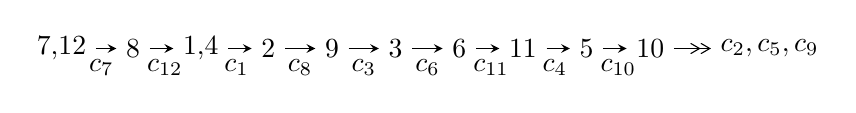
\begin{tikzpicture}[x=23pt, y=7pt]
	% node
	\node (A0) at (-1/8, 0) {7,12};
	\node (A1) at (1, 0) {8};
	\node (A2) at (33/16, 0) {1,4};
	\node (A3) at (25/8, 0) {2};
	\node (A4) at (33/8, 0) {9};
	\node (A5) at (41/8, 0) {3};
	\node (A6) at (49/8, 0) {6};
	\node (A7) at (57/8, 0) {11};
	\node (A8) at (65/8, 0) {5};
	\node (A9) at (73/8, 0) {10};
	\node (C1) at (1/2, -1) {$c_{7}$};
	\node (C2) at (3/2, -1) {$c_{12}$};
	\node (C3) at (21/8, -1) {$c_{1}$};
	\node (C4) at (29/8, -1) {$c_{8}$};
	\node (C5) at (37/8, -1) {$c_{3}$};
	\node (C6) at (45/8, -1) {$c_{6}$};
	\node (C7) at (53/8, -1) {$c_{11}$};
	\node (C8) at (61/8, -1) {$c_{4}$};
	\node (C9) at (69/8, -1) {$c_{10}$};
	\node (A10) at (11, 0) {$c_{2},c_{5},c_{9}$};

	% edge
	\draw[->,>=stealth]	
	(A0) edge (A1) (A1) edge (A2) (A2) edge (A3) (A3) edge (A4) (A4) edge (A5) (A5) edge (A6) (A6) edge (A7) (A7) edge (A8) (A8) edge (A9) ;
	\draw[->>,>={angle 60}]	
	(A9) edge (A10);
\end{tikzpicture} \\ 

\end{tabular} \\

\footnotetext{
The image of knot diagram is generated by the software ``\textbf{Draw programme}" developed by Andrew Bartholomew(\url{http://www.layer8.co.uk/maths/draw/index.htm\#Running-draw}), where we modified some parts for our purpose(\url{https://github.com/CATsTAILs/LinksPainter}).
}\phantom \\ \newline 
\centering \textbf{Ideals for irreducible components\footnotemark of $X_{\text{par}}$} 
 
\begin{align*}
I^u_{1}&=\langle 
6.39446\times10^{159} u^{107}-3.76803\times10^{159} u^{106}+\cdots+6.12809\times10^{158} b+2.51906\times10^{161},\\
\phantom{I^u_{1}}&\phantom{= \langle  }-1.20288\times10^{161} u^{107}+4.35929\times10^{160} u^{106}+\cdots+1.16434\times10^{160} a-4.81370\times10^{162},\\
\phantom{I^u_{1}}&\phantom{= \langle  }u^{108}-64 u^{106}+\cdots+79 u+19\rangle \\
I^u_{2}&=\langle 
-6 u^{19}+5 u^{18}+\cdots+b+11,\;-22 u^{19}+25 u^{18}+\cdots+a+65,\;u^{20}- u^{19}+\cdots-3 u-1\rangle \\
\\
\end{align*}
\raggedright * 2 irreducible components of $\dim_{\mathbb{C}}=0$, with total 128 representations.\\
\footnotetext{All coefficients of polynomials are rational numbers. But the coefficients are sometimes approximated in decimal forms when there is not enough margin.}
\newpage
\renewcommand{\arraystretch}{1}
\centering \section*{I. $I^u_{1}= \langle 6.39\times10^{159} u^{107}-3.77\times10^{159} u^{106}+\cdots+6.13\times10^{158} b+2.52\times10^{161},\;-1.20\times10^{161} u^{107}+4.36\times10^{160} u^{106}+\cdots+1.16\times10^{160} a-4.81\times10^{162},\;u^{108}-64 u^{106}+\cdots+79 u+19 \rangle$}
\flushleft \textbf{(i) Arc colorings}\\
\begin{tabular}{m{7pt} m{180pt} m{7pt} m{180pt} }
\flushright $a_{7}=$&$\begin{pmatrix}1\\0\end{pmatrix}$ \\
\flushright $a_{12}=$&$\begin{pmatrix}0\\u\end{pmatrix}$ \\
\flushright $a_{8}=$&$\begin{pmatrix}1\\u^2\end{pmatrix}$ \\
\flushright $a_{1}=$&$\begin{pmatrix}- u\\- u^3+u\end{pmatrix}$ \\
\flushright $a_{4}=$&$\begin{pmatrix}10.3310 u^{107}-3.74401 u^{106}+\cdots+793.996 u+413.428\\-10.4347 u^{107}+6.14879 u^{106}+\cdots-929.658 u-411.068\end{pmatrix}$ \\
\flushright $a_{2}=$&$\begin{pmatrix}-2.98176 u^{107}+2.93862 u^{106}+\cdots-411.821 u-156.791\\-1.87036 u^{107}+1.63181 u^{106}+\cdots-260.056 u-126.652\end{pmatrix}$ \\
\flushright $a_{9}=$&$\begin{pmatrix}- u^2+1\\- u^4+2 u^2\end{pmatrix}$ \\
\flushright $a_{3}=$&$\begin{pmatrix}19.0569 u^{107}-8.18342 u^{106}+\cdots+1516.78 u+752.274\\-5.23619 u^{107}+3.46950 u^{106}+\cdots-506.976 u-215.183\end{pmatrix}$ \\
\flushright $a_{6}=$&$\begin{pmatrix}13.4025 u^{107}-6.62774 u^{106}+\cdots+1005.37 u+465.422\\-3.69603 u^{107}+1.87222 u^{106}+\cdots-362.917 u-184.182\end{pmatrix}$ \\
\flushright $a_{11}=$&$\begin{pmatrix}u\\u\end{pmatrix}$ \\
\flushright $a_{5}=$&$\begin{pmatrix}15.0580 u^{107}-6.03524 u^{106}+\cdots+1180.98 u+601.392\\-5.70771 u^{107}+3.85755 u^{106}+\cdots-542.675 u-223.105\end{pmatrix}$ \\
\flushright $a_{10}=$&$\begin{pmatrix}57.1117 u^{107}-29.2858 u^{106}+\cdots+4525.00 u+1962.94\\-6.37163 u^{107}+4.48054 u^{106}+\cdots-574.058 u-265.244\end{pmatrix}$\\&\end{tabular}
\flushleft \textbf{(ii) Obstruction class $= -1$}\\~\\
\flushleft \textbf{(iii) Cusp Shapes $= 2474.05 u^{107}-1304.36 u^{106}+\cdots+202505. u+89977.7$}\\~\\
\newpage\renewcommand{\arraystretch}{1}
\flushleft \textbf{(iv) u-Polynomials at the component}\newline \\
\begin{tabular}{m{50pt}|m{274pt}}
Crossings & \hspace{64pt}u-Polynomials at each crossing \\
\hline $$\begin{aligned}c_{1}\end{aligned}$$&$\begin{aligned}
&u^{108}+3 u^{107}+\cdots-14150 u-877
\end{aligned}$\\
\hline $$\begin{aligned}c_{2}\end{aligned}$$&$\begin{aligned}
&u^{108}-3 u^{107}+\cdots-263 u+863
\end{aligned}$\\
\hline $$\begin{aligned}c_{3}\end{aligned}$$&$\begin{aligned}
&u^{108}-2 u^{107}+\cdots-146927 u+6859
\end{aligned}$\\
\hline $$\begin{aligned}c_{4},c_{10}\end{aligned}$$&$\begin{aligned}
&u^{108}-2 u^{107}+\cdots+41712 u+7342
\end{aligned}$\\
\hline $$\begin{aligned}c_{5}\end{aligned}$$&$\begin{aligned}
&u^{108}+9 u^{106}+\cdots-13 u+1
\end{aligned}$\\
\hline $$\begin{aligned}c_{6}\end{aligned}$$&$\begin{aligned}
&u^{108}-3 u^{107}+\cdots+210 u+50
\end{aligned}$\\
\hline $$\begin{aligned}c_{7},c_{8},c_{11}\\c_{12}\end{aligned}$$&$\begin{aligned}
&u^{108}-64 u^{106}+\cdots+79 u+19
\end{aligned}$\\
\hline $$\begin{aligned}c_{9}\end{aligned}$$&$\begin{aligned}
&u^{108}-6 u^{107}+\cdots-26 u-1
\end{aligned}$\\
\hline
\end{tabular}\\~\\
\newpage\renewcommand{\arraystretch}{1}
\flushleft \textbf{(v) Riley Polynomials at the component}\newline \\
\begin{tabular}{m{50pt}|m{274pt}}
Crossings & \hspace{64pt}Riley Polynomials at each crossing \\
\hline $$\begin{aligned}c_{1}\end{aligned}$$&$\begin{aligned}
&y^{108}-23 y^{107}+\cdots-277829984 y+769129
\end{aligned}$\\
\hline $$\begin{aligned}c_{2}\end{aligned}$$&$\begin{aligned}
&y^{108}+23 y^{107}+\cdots+28915549 y+744769
\end{aligned}$\\
\hline $$\begin{aligned}c_{3}\end{aligned}$$&$\begin{aligned}
&y^{108}+24 y^{107}+\cdots-8465521839 y+47045881
\end{aligned}$\\
\hline $$\begin{aligned}c_{4},c_{10}\end{aligned}$$&$\begin{aligned}
&y^{108}+62 y^{107}+\cdots+2759081080 y+53904964
\end{aligned}$\\
\hline $$\begin{aligned}c_{5}\end{aligned}$$&$\begin{aligned}
&y^{108}+18 y^{107}+\cdots-117 y+1
\end{aligned}$\\
\hline $$\begin{aligned}c_{6}\end{aligned}$$&$\begin{aligned}
&y^{108}+7 y^{107}+\cdots-182700 y+2500
\end{aligned}$\\
\hline $$\begin{aligned}c_{7},c_{8},c_{11}\\c_{12}\end{aligned}$$&$\begin{aligned}
&y^{108}-128 y^{107}+\cdots-7001 y+361
\end{aligned}$\\
\hline $$\begin{aligned}c_{9}\end{aligned}$$&$\begin{aligned}
&y^{108}+2 y^{107}+\cdots-400 y+1
\end{aligned}$\\
\hline
\end{tabular}\\~\\
\newpage\flushleft \textbf{(vi) Complex Volumes and Cusp Shapes}
$$\begin{array}{c|c|c}  
\text{Solutions to }I^u_{1}& \I (\text{vol} + \sqrt{-1}CS) & \text{Cusp shape}\\
 \hline 
\begin{aligned}
u &= -0.918403 + 0.363047 I \\
a &= \phantom{-}0.577687 + 0.075821 I \\
b &= \phantom{-}1.29762 - 0.97342 I\end{aligned}
 & -0.68898 + 5.29923 I & \phantom{-0.000000 } 0 \\ \hline\begin{aligned}
u &= -0.918403 - 0.363047 I \\
a &= \phantom{-}0.577687 - 0.075821 I \\
b &= \phantom{-}1.29762 + 0.97342 I\end{aligned}
 & -0.68898 - 5.29923 I & \phantom{-0.000000 } 0 \\ \hline\begin{aligned}
u &= -0.786840 + 0.594679 I \\
a &= -0.360188 - 0.273117 I \\
b &= -1.65851 + 0.51392 I\end{aligned}
 & \phantom{-}0.8477 + 14.7408 I & \phantom{-0.000000 } 0 \\ \hline\begin{aligned}
u &= -0.786840 - 0.594679 I \\
a &= -0.360188 + 0.273117 I \\
b &= -1.65851 - 0.51392 I\end{aligned}
 & \phantom{-}0.8477 - 14.7408 I & \phantom{-0.000000 } 0 \\ \hline\begin{aligned}
u &= -0.853224 + 0.471994 I \\
a &= -0.082684 - 0.260349 I \\
b &= -1.086620 - 0.376320 I\end{aligned}
 & -3.71442 - 1.11666 I & \phantom{-0.000000 } 0 \\ \hline\begin{aligned}
u &= -0.853224 - 0.471994 I \\
a &= -0.082684 + 0.260349 I \\
b &= -1.086620 + 0.376320 I\end{aligned}
 & -3.71442 + 1.11666 I & \phantom{-0.000000 } 0 \\ \hline\begin{aligned}
u &= \phantom{-}0.762919 + 0.594989 I \\
a &= \phantom{-}0.127443 - 0.379906 I \\
b &= \phantom{-}1.48454 + 0.30248 I\end{aligned}
 & \phantom{-}2.37811 - 6.64794 I & \phantom{-0.000000 } 0 \\ \hline\begin{aligned}
u &= \phantom{-}0.762919 - 0.594989 I \\
a &= \phantom{-}0.127443 + 0.379906 I \\
b &= \phantom{-}1.48454 - 0.30248 I\end{aligned}
 & \phantom{-}2.37811 + 6.64794 I & \phantom{-0.000000 } 0 \\ \hline\begin{aligned}
u &= \phantom{-}0.828146 + 0.461143 I \\
a &= -0.074938 + 0.356052 I \\
b &= \phantom{-}1.048180 - 0.185516 I\end{aligned}
 & -3.68598 - 8.69698 I & \phantom{-0.000000 } 0 \\ \hline\begin{aligned}
u &= \phantom{-}0.828146 - 0.461143 I \\
a &= -0.074938 - 0.356052 I \\
b &= \phantom{-}1.048180 + 0.185516 I\end{aligned}
 & -3.68598 + 8.69698 I & \phantom{-0.000000 } 0\\
 \hline 
 \end{array}$$\newpage$$\begin{array}{c|c|c}  
\text{Solutions to }I^u_{1}& \I (\text{vol} + \sqrt{-1}CS) & \text{Cusp shape}\\
 \hline 
\begin{aligned}
u &= -0.839992 + 0.662463 I \\
a &= \phantom{-}0.336973 + 0.212786 I \\
b &= \phantom{-}1.062600 - 0.510318 I\end{aligned}
 & \phantom{-}1.14032 + 5.01007 I & \phantom{-0.000000 } 0 \\ \hline\begin{aligned}
u &= -0.839992 - 0.662463 I \\
a &= \phantom{-}0.336973 - 0.212786 I \\
b &= \phantom{-}1.062600 + 0.510318 I\end{aligned}
 & \phantom{-}1.14032 - 5.01007 I & \phantom{-0.000000 } 0 \\ \hline\begin{aligned}
u &= -0.135219 + 0.871002 I \\
a &= -0.508112 + 0.365104 I \\
b &= \phantom{-}0.632779 + 0.185856 I\end{aligned}
 & \phantom{-}3.29458 + 0.06012 I & \phantom{-0.000000 } 0 \\ \hline\begin{aligned}
u &= -0.135219 - 0.871002 I \\
a &= -0.508112 - 0.365104 I \\
b &= \phantom{-}0.632779 - 0.185856 I\end{aligned}
 & \phantom{-}3.29458 - 0.06012 I & \phantom{-0.000000 } 0 \\ \hline\begin{aligned}
u &= \phantom{-}0.816794 + 0.324059 I \\
a &= -0.196676 - 0.789532 I \\
b &= -0.046523 - 0.614863 I\end{aligned}
 & -1.09335 - 4.09841 I & \phantom{-0.000000 } 0 \\ \hline\begin{aligned}
u &= \phantom{-}0.816794 - 0.324059 I \\
a &= -0.196676 + 0.789532 I \\
b &= -0.046523 + 0.614863 I\end{aligned}
 & -1.09335 + 4.09841 I & \phantom{-0.000000 } 0 \\ \hline\begin{aligned}
u &= \phantom{-}0.745079 + 0.455136 I \\
a &= -0.599572 - 0.052001 I \\
b &= -1.57915 - 0.82326 I\end{aligned}
 & -1.44059 - 6.30070 I & \phantom{-0.000000 } 0 \\ \hline\begin{aligned}
u &= \phantom{-}0.745079 - 0.455136 I \\
a &= -0.599572 + 0.052001 I \\
b &= -1.57915 + 0.82326 I\end{aligned}
 & -1.44059 + 6.30070 I & \phantom{-0.000000 } 0 \\ \hline\begin{aligned}
u &= -0.763932 + 0.347374 I \\
a &= \phantom{-}0.391757 - 0.366806 I \\
b &= \phantom{-}0.259733 + 0.554449 I\end{aligned}
 & -2.10240 + 0.07367 I & \phantom{-0.000000 } 0 \\ \hline\begin{aligned}
u &= -0.763932 - 0.347374 I \\
a &= \phantom{-}0.391757 + 0.366806 I \\
b &= \phantom{-}0.259733 - 0.554449 I\end{aligned}
 & -2.10240 - 0.07367 I & \phantom{-0.000000 } 0\\
 \hline 
 \end{array}$$\newpage$$\begin{array}{c|c|c}  
\text{Solutions to }I^u_{1}& \I (\text{vol} + \sqrt{-1}CS) & \text{Cusp shape}\\
 \hline 
\begin{aligned}
u &= \phantom{-}1.115360 + 0.391127 I \\
a &= -0.069494 + 0.571612 I \\
b &= -0.009646 - 0.486385 I\end{aligned}
 & -1.21891 + 6.13662 I & \phantom{-0.000000 } 0 \\ \hline\begin{aligned}
u &= \phantom{-}1.115360 - 0.391127 I \\
a &= -0.069494 - 0.571612 I \\
b &= -0.009646 + 0.486385 I\end{aligned}
 & -1.21891 - 6.13662 I & \phantom{-0.000000 } 0 \\ \hline\begin{aligned}
u &= \phantom{-}0.792577 + 0.183240 I \\
a &= -0.528779 - 0.502606 I \\
b &= -1.251760 - 0.258832 I\end{aligned}
 & -4.28634 - 1.95164 I & \phantom{-0.000000 } 0 \\ \hline\begin{aligned}
u &= \phantom{-}0.792577 - 0.183240 I \\
a &= -0.528779 + 0.502606 I \\
b &= -1.251760 + 0.258832 I\end{aligned}
 & -4.28634 + 1.95164 I & \phantom{-0.000000 } 0 \\ \hline\begin{aligned}
u &= \phantom{-}0.221271 + 0.765584 I \\
a &= -0.509266 - 0.902262 I \\
b &= \phantom{-}0.705595 + 0.169000 I\end{aligned}
 & \phantom{-}4.04452 + 2.10493 I & \phantom{-0.000000 } 0 \\ \hline\begin{aligned}
u &= \phantom{-}0.221271 - 0.765584 I \\
a &= -0.509266 + 0.902262 I \\
b &= \phantom{-}0.705595 - 0.169000 I\end{aligned}
 & \phantom{-}4.04452 - 2.10493 I & \phantom{-0.000000 } 0 \\ \hline\begin{aligned}
u &= -0.160991 + 0.770485 I \\
a &= \phantom{-}0.754805 - 1.020410 I \\
b &= -0.743086 - 0.054824 I\end{aligned}
 & \phantom{-}2.73787 - 10.19870 I & \phantom{-0.000000 } 0 \\ \hline\begin{aligned}
u &= -0.160991 - 0.770485 I \\
a &= \phantom{-}0.754805 + 1.020410 I \\
b &= -0.743086 + 0.054824 I\end{aligned}
 & \phantom{-}2.73787 + 10.19870 I & \phantom{-0.000000 } 0 \\ \hline\begin{aligned}
u &= \phantom{-}0.542523 + 0.538416 I \\
a &= -0.539993 + 0.936976 I \\
b &= -1.50096 + 0.19417 I\end{aligned}
 & -1.94334 - 1.86285 I & \phantom{-0.000000 } 0 \\ \hline\begin{aligned}
u &= \phantom{-}0.542523 - 0.538416 I \\
a &= -0.539993 - 0.936976 I \\
b &= -1.50096 - 0.19417 I\end{aligned}
 & -1.94334 + 1.86285 I & \phantom{-0.000000 } 0\\
 \hline 
 \end{array}$$\newpage$$\begin{array}{c|c|c}  
\text{Solutions to }I^u_{1}& \I (\text{vol} + \sqrt{-1}CS) & \text{Cusp shape}\\
 \hline 
\begin{aligned}
u &= -0.734335 + 0.204776 I \\
a &= \phantom{-}0.572466 + 0.621429 I \\
b &= -0.570960 - 0.128398 I\end{aligned}
 & -0.806750 + 0.415425 I & \phantom{-0.000000 } 0 \\ \hline\begin{aligned}
u &= -0.734335 - 0.204776 I \\
a &= \phantom{-}0.572466 - 0.621429 I \\
b &= -0.570960 + 0.128398 I\end{aligned}
 & -0.806750 - 0.415425 I & \phantom{-0.000000 } 0 \\ \hline\begin{aligned}
u &= -0.673601 + 0.348591 I \\
a &= \phantom{-}0.529252 - 0.790567 I \\
b &= \phantom{-}0.972439 + 0.173848 I\end{aligned}
 & -3.05293 + 2.31643 I & \phantom{-0.000000 } 0 \\ \hline\begin{aligned}
u &= -0.673601 - 0.348591 I \\
a &= \phantom{-}0.529252 + 0.790567 I \\
b &= \phantom{-}0.972439 - 0.173848 I\end{aligned}
 & -3.05293 - 2.31643 I & \phantom{-0.000000 } 0 \\ \hline\begin{aligned}
u &= \phantom{-}1.175480 + 0.414874 I \\
a &= \phantom{-}0.103995 - 0.595442 I \\
b &= \phantom{-}0.479884 + 0.042072 I\end{aligned}
 & -0.72700 - 4.62038 I & \phantom{-0.000000 } 0 \\ \hline\begin{aligned}
u &= \phantom{-}1.175480 - 0.414874 I \\
a &= \phantom{-}0.103995 + 0.595442 I \\
b &= \phantom{-}0.479884 - 0.042072 I\end{aligned}
 & -0.72700 + 4.62038 I & \phantom{-0.000000 } 0 \\ \hline\begin{aligned}
u &= \phantom{-}0.337393 + 0.638153 I \\
a &= -0.936417 - 0.482034 I \\
b &= \phantom{-}0.657396 + 0.231964 I\end{aligned}
 & \phantom{-}3.17800 - 2.10286 I & \phantom{-0.000000 } 0 \\ \hline\begin{aligned}
u &= \phantom{-}0.337393 - 0.638153 I \\
a &= -0.936417 + 0.482034 I \\
b &= \phantom{-}0.657396 - 0.231964 I\end{aligned}
 & \phantom{-}3.17800 + 2.10286 I & \phantom{-0.000000 } 0 \\ \hline\begin{aligned}
u &= \phantom{-}0.581607 + 0.356113 I \\
a &= \phantom{-}0.268997 + 0.217922 I \\
b &= -1.41217 - 0.94149 I\end{aligned}
 & \phantom{-}3.56570 - 6.80593 I & \phantom{-0.000000 } 0 \\ \hline\begin{aligned}
u &= \phantom{-}0.581607 - 0.356113 I \\
a &= \phantom{-}0.268997 - 0.217922 I \\
b &= -1.41217 + 0.94149 I\end{aligned}
 & \phantom{-}3.56570 + 6.80593 I & \phantom{-0.000000 } 0\\
 \hline 
 \end{array}$$\newpage$$\begin{array}{c|c|c}  
\text{Solutions to }I^u_{1}& \I (\text{vol} + \sqrt{-1}CS) & \text{Cusp shape}\\
 \hline 
\begin{aligned}
u &= -0.004677 + 0.664850 I \\
a &= -0.193937 - 1.179350 I \\
b &= -0.270651 + 0.253195 I\end{aligned}
 & -1.17764 + 4.94781 I & \phantom{-0.000000 } 0 \\ \hline\begin{aligned}
u &= -0.004677 - 0.664850 I \\
a &= -0.193937 + 1.179350 I \\
b &= -0.270651 - 0.253195 I\end{aligned}
 & -1.17764 - 4.94781 I & \phantom{-0.000000 } 0 \\ \hline\begin{aligned}
u &= -1.318830 + 0.302141 I \\
a &= \phantom{-}0.405046 + 0.324159 I \\
b &= \phantom{-}0.210817 - 0.448074 I\end{aligned}
 & -0.71202 + 1.74500 I & \phantom{-0.000000 } 0 \\ \hline\begin{aligned}
u &= -1.318830 - 0.302141 I \\
a &= \phantom{-}0.405046 - 0.324159 I \\
b &= \phantom{-}0.210817 + 0.448074 I\end{aligned}
 & -0.71202 - 1.74500 I & \phantom{-0.000000 } 0 \\ \hline\begin{aligned}
u &= \phantom{-}0.473407 + 0.403433 I \\
a &= \phantom{-}0.191460 - 1.124820 I \\
b &= \phantom{-}1.38625 + 0.38967 I\end{aligned}
 & \phantom{-}3.27491 - 1.44689 I & \phantom{-0.000000 } 0 \\ \hline\begin{aligned}
u &= \phantom{-}0.473407 - 0.403433 I \\
a &= \phantom{-}0.191460 + 1.124820 I \\
b &= \phantom{-}1.38625 - 0.38967 I\end{aligned}
 & \phantom{-}3.27491 + 1.44689 I & \phantom{-0.000000 } 0 \\ \hline\begin{aligned}
u &= \phantom{-}0.449380 + 0.427340 I \\
a &= -0.30281 - 1.54482 I \\
b &= \phantom{-}1.230100 - 0.077357 I\end{aligned}
 & \phantom{-}3.34419 - 1.57237 I & \phantom{-0.000000 } 0 \\ \hline\begin{aligned}
u &= \phantom{-}0.449380 - 0.427340 I \\
a &= -0.30281 + 1.54482 I \\
b &= \phantom{-}1.230100 + 0.077357 I\end{aligned}
 & \phantom{-}3.34419 + 1.57237 I & \phantom{-0.000000 } 0 \\ \hline\begin{aligned}
u &= -0.543074 + 0.265773 I \\
a &= -1.073620 - 0.183651 I \\
b &= -1.67123 + 1.50600 I\end{aligned}
 & \phantom{-}3.02271 - 3.50835 I & \phantom{-0.000000 } 0 \\ \hline\begin{aligned}
u &= -0.543074 - 0.265773 I \\
a &= -1.073620 + 0.183651 I \\
b &= -1.67123 - 1.50600 I\end{aligned}
 & \phantom{-}3.02271 + 3.50835 I & \phantom{-0.000000 } 0\\
 \hline 
 \end{array}$$\newpage$$\begin{array}{c|c|c}  
\text{Solutions to }I^u_{1}& \I (\text{vol} + \sqrt{-1}CS) & \text{Cusp shape}\\
 \hline 
\begin{aligned}
u &= -0.561967 + 0.148339 I \\
a &= \phantom{-}0.06600 + 2.18752 I \\
b &= \phantom{-}1.063990 - 0.687409 I\end{aligned}
 & \phantom{-}1.153670 + 0.568402 I & -18.5278 + 5.1996 I \\ \hline\begin{aligned}
u &= -0.561967 - 0.148339 I \\
a &= \phantom{-}0.06600 - 2.18752 I \\
b &= \phantom{-}1.063990 + 0.687409 I\end{aligned}
 & \phantom{-}1.153670 - 0.568402 I & -18.5278 - 5.1996 I \\ \hline\begin{aligned}
u &= \phantom{-}0.085437 + 0.562730 I \\
a &= \phantom{-}1.30050 + 1.06453 I \\
b &= -0.344796 + 0.356638 I\end{aligned}
 & \phantom{-}0.48204 + 2.83082 I & -6.00000 - 4.98877 I \\ \hline\begin{aligned}
u &= \phantom{-}0.085437 - 0.562730 I \\
a &= \phantom{-}1.30050 - 1.06453 I \\
b &= -0.344796 - 0.356638 I\end{aligned}
 & \phantom{-}0.48204 - 2.83082 I & -6.00000 + 4.98877 I \\ \hline\begin{aligned}
u &= -0.487598 + 0.197242 I \\
a &= \phantom{-}0.52968 - 3.54305 I \\
b &= -0.64961 - 1.36649 I\end{aligned}
 & \phantom{-}3.29846 + 5.31621 I & -6.6460 - 12.8715 I \\ \hline\begin{aligned}
u &= -0.487598 - 0.197242 I \\
a &= \phantom{-}0.52968 + 3.54305 I \\
b &= -0.64961 + 1.36649 I\end{aligned}
 & \phantom{-}3.29846 - 5.31621 I & -6.6460 + 12.8715 I \\ \hline\begin{aligned}
u &= -0.524996\phantom{ +0.000000I} \\
a &= -3.34733\phantom{ +0.000000I} \\
b &= \phantom{-}2.70406\phantom{ +0.000000I}\end{aligned}
 & \phantom{-}0.861575\phantom{ +0.000000I} & -721.720\phantom{ +0.000000I} \\ \hline\begin{aligned}
u &= -1.51099 + 0.01392 I \\
a &= \phantom{-}0.415611 - 0.142159 I \\
b &= \phantom{-}0.573366 + 0.852056 I\end{aligned}
 & -1.75741 - 3.30179 I & \phantom{-0.000000 } 0 \\ \hline\begin{aligned}
u &= -1.51099 - 0.01392 I \\
a &= \phantom{-}0.415611 + 0.142159 I \\
b &= \phantom{-}0.573366 - 0.852056 I\end{aligned}
 & -1.75741 + 3.30179 I & \phantom{-0.000000 } 0 \\ \hline\begin{aligned}
u &= -0.478642\phantom{ +0.000000I} \\
a &= \phantom{-}0.759788\phantom{ +0.000000I} \\
b &= -0.383924\phantom{ +0.000000I}\end{aligned}
 & -0.850740\phantom{ +0.000000I} & -12.2080\phantom{ +0.000000I}\\
 \hline 
 \end{array}$$\newpage$$\begin{array}{c|c|c}  
\text{Solutions to }I^u_{1}& \I (\text{vol} + \sqrt{-1}CS) & \text{Cusp shape}\\
 \hline 
\begin{aligned}
u &= \phantom{-}0.322815 + 0.350066 I \\
a &= \phantom{-}1.39524 + 2.51421 I \\
b &= -0.166714 - 0.009266 I\end{aligned}
 & \phantom{-}4.31901 + 4.18133 I & -0.636621 + 0.682075 I \\ \hline\begin{aligned}
u &= \phantom{-}0.322815 - 0.350066 I \\
a &= \phantom{-}1.39524 - 2.51421 I \\
b &= -0.166714 + 0.009266 I\end{aligned}
 & \phantom{-}4.31901 - 4.18133 I & -0.636621 - 0.682075 I \\ \hline\begin{aligned}
u &= -1.52286 + 0.07536 I \\
a &= \phantom{-}1.46969 + 0.87081 I \\
b &= \phantom{-}1.58641 + 0.00893 I\end{aligned}
 & -3.21753 + 3.18908 I & \phantom{-0.000000 } 0 \\ \hline\begin{aligned}
u &= -1.52286 - 0.07536 I \\
a &= \phantom{-}1.46969 - 0.87081 I \\
b &= \phantom{-}1.58641 - 0.00893 I\end{aligned}
 & -3.21753 - 3.18908 I & \phantom{-0.000000 } 0 \\ \hline\begin{aligned}
u &= \phantom{-}1.54723\phantom{ +0.000000I} \\
a &= -1.50376\phantom{ +0.000000I} \\
b &= -2.03839\phantom{ +0.000000I}\end{aligned}
 & -7.67325\phantom{ +0.000000I} & \phantom{-0.000000 } 0 \\ \hline\begin{aligned}
u &= -1.54915 + 0.07118 I \\
a &= \phantom{-}2.25525 + 0.03732 I \\
b &= \phantom{-}2.37551 - 0.62818 I\end{aligned}
 & -3.55685 + 2.93173 I & \phantom{-0.000000 } 0 \\ \hline\begin{aligned}
u &= -1.54915 - 0.07118 I \\
a &= \phantom{-}2.25525 - 0.03732 I \\
b &= \phantom{-}2.37551 + 0.62818 I\end{aligned}
 & -3.55685 - 2.93173 I & \phantom{-0.000000 } 0 \\ \hline\begin{aligned}
u &= \phantom{-}1.56910 + 0.05756 I \\
a &= -2.77571 - 1.20477 I \\
b &= -2.80809 - 1.79704 I\end{aligned}
 & -4.22369 + 2.41374 I & \phantom{-0.000000 } 0 \\ \hline\begin{aligned}
u &= \phantom{-}1.56910 - 0.05756 I \\
a &= -2.77571 + 1.20477 I \\
b &= -2.80809 + 1.79704 I\end{aligned}
 & -4.22369 - 2.41374 I & \phantom{-0.000000 } 0 \\ \hline\begin{aligned}
u &= \phantom{-}1.57523 + 0.04067 I \\
a &= -0.34969 + 1.94842 I \\
b &= -0.442055 + 1.066160 I\end{aligned}
 & -3.90930 - 6.07655 I & \phantom{-0.000000 } 0\\
 \hline 
 \end{array}$$\newpage$$\begin{array}{c|c|c}  
\text{Solutions to }I^u_{1}& \I (\text{vol} + \sqrt{-1}CS) & \text{Cusp shape}\\
 \hline 
\begin{aligned}
u &= \phantom{-}1.57523 - 0.04067 I \\
a &= -0.34969 - 1.94842 I \\
b &= -0.442055 - 1.066160 I\end{aligned}
 & -3.90930 + 6.07655 I & \phantom{-0.000000 } 0 \\ \hline\begin{aligned}
u &= -1.57034 + 0.16360 I \\
a &= -1.97014 - 0.95650 I \\
b &= -2.20061 - 0.32678 I\end{aligned}
 & -9.09144 + 4.42081 I & \phantom{-0.000000 } 0 \\ \hline\begin{aligned}
u &= -1.57034 - 0.16360 I \\
a &= -1.97014 + 0.95650 I \\
b &= -2.20061 + 0.32678 I\end{aligned}
 & -9.09144 - 4.42081 I & \phantom{-0.000000 } 0 \\ \hline\begin{aligned}
u &= -1.57717 + 0.08329 I \\
a &= -2.44275 + 0.93501 I \\
b &= -2.95985 + 1.70623 I\end{aligned}
 & -3.80592 + 8.32471 I & \phantom{-0.000000 } 0 \\ \hline\begin{aligned}
u &= -1.57717 - 0.08329 I \\
a &= -2.44275 - 0.93501 I \\
b &= -2.95985 - 1.70623 I\end{aligned}
 & -3.80592 - 8.32471 I & \phantom{-0.000000 } 0 \\ \hline\begin{aligned}
u &= \phantom{-}1.58453\phantom{ +0.000000I} \\
a &= \phantom{-}3.66567\phantom{ +0.000000I} \\
b &= \phantom{-}5.23316\phantom{ +0.000000I}\end{aligned}
 & -6.52398\phantom{ +0.000000I} & \phantom{-0.000000 } 0 \\ \hline\begin{aligned}
u &= \phantom{-}1.59172 + 0.03587 I \\
a &= \phantom{-}1.48460 + 0.91593 I \\
b &= \phantom{-}1.69763 + 2.07886 I\end{aligned}
 & -6.36818 - 1.20710 I & \phantom{-0.000000 } 0 \\ \hline\begin{aligned}
u &= \phantom{-}1.59172 - 0.03587 I \\
a &= \phantom{-}1.48460 - 0.91593 I \\
b &= \phantom{-}1.69763 - 2.07886 I\end{aligned}
 & -6.36818 + 1.20710 I & \phantom{-0.000000 } 0 \\ \hline\begin{aligned}
u &= \phantom{-}0.013147 + 0.404692 I \\
a &= \phantom{-}0.916367 - 0.639370 I \\
b &= \phantom{-}0.435184 + 0.458824 I\end{aligned}
 & \phantom{-}1.21199 + 1.56615 I & -0.45773 - 2.46701 I \\ \hline\begin{aligned}
u &= \phantom{-}0.013147 - 0.404692 I \\
a &= \phantom{-}0.916367 + 0.639370 I \\
b &= \phantom{-}0.435184 - 0.458824 I\end{aligned}
 & \phantom{-}1.21199 - 1.56615 I & -0.45773 + 2.46701 I\\
 \hline 
 \end{array}$$\newpage$$\begin{array}{c|c|c}  
\text{Solutions to }I^u_{1}& \I (\text{vol} + \sqrt{-1}CS) & \text{Cusp shape}\\
 \hline 
\begin{aligned}
u &= -0.139404 + 0.368779 I \\
a &= \phantom{-}0.82345 + 1.47280 I \\
b &= -0.221813 + 0.391507 I\end{aligned}
 & -1.58343 + 0.26531 I & -8.98911 - 1.46511 I \\ \hline\begin{aligned}
u &= -0.139404 - 0.368779 I \\
a &= \phantom{-}0.82345 - 1.47280 I \\
b &= -0.221813 - 0.391507 I\end{aligned}
 & -1.58343 - 0.26531 I & -8.98911 + 1.46511 I \\ \hline\begin{aligned}
u &= \phantom{-}1.60487 + 0.09478 I \\
a &= \phantom{-}1.89473 - 0.69782 I \\
b &= \phantom{-}2.32906 - 1.10540 I\end{aligned}
 & -10.87800 - 3.94093 I & \phantom{-0.000000 } 0 \\ \hline\begin{aligned}
u &= \phantom{-}1.60487 - 0.09478 I \\
a &= \phantom{-}1.89473 + 0.69782 I \\
b &= \phantom{-}2.32906 + 1.10540 I\end{aligned}
 & -10.87800 + 3.94093 I & \phantom{-0.000000 } 0 \\ \hline\begin{aligned}
u &= \phantom{-}1.62125 + 0.10554 I \\
a &= \phantom{-}0.835187 - 0.849590 I \\
b &= \phantom{-}1.03381 - 1.24999 I\end{aligned}
 & -10.25420 - 1.81805 I & \phantom{-0.000000 } 0 \\ \hline\begin{aligned}
u &= \phantom{-}1.62125 - 0.10554 I \\
a &= \phantom{-}0.835187 + 0.849590 I \\
b &= \phantom{-}1.03381 + 1.24999 I\end{aligned}
 & -10.25420 + 1.81805 I & \phantom{-0.000000 } 0 \\ \hline\begin{aligned}
u &= -1.62134 + 0.13055 I \\
a &= -2.66168 + 0.40813 I \\
b &= -2.99226 + 1.01910 I\end{aligned}
 & -9.51933 + 8.50404 I & \phantom{-0.000000 } 0 \\ \hline\begin{aligned}
u &= -1.62134 - 0.13055 I \\
a &= -2.66168 - 0.40813 I \\
b &= -2.99226 - 1.01910 I\end{aligned}
 & -9.51933 - 8.50404 I & \phantom{-0.000000 } 0 \\ \hline\begin{aligned}
u &= \phantom{-}1.63391 + 0.06790 I \\
a &= -1.54583 + 0.66573 I \\
b &= -2.34433 + 1.12590 I\end{aligned}
 & -9.10384 - 1.49738 I & \phantom{-0.000000 } 0 \\ \hline\begin{aligned}
u &= \phantom{-}1.63391 - 0.06790 I \\
a &= -1.54583 - 0.66573 I \\
b &= -2.34433 - 1.12590 I\end{aligned}
 & -9.10384 + 1.49738 I & \phantom{-0.000000 } 0\\
 \hline 
 \end{array}$$\newpage$$\begin{array}{c|c|c}  
\text{Solutions to }I^u_{1}& \I (\text{vol} + \sqrt{-1}CS) & \text{Cusp shape}\\
 \hline 
\begin{aligned}
u &= -1.63138 + 0.17483 I \\
a &= \phantom{-}2.10964 + 0.04433 I \\
b &= \phantom{-}2.63177 - 0.78645 I\end{aligned}
 & -5.73693 + 9.55495 I & \phantom{-0.000000 } 0 \\ \hline\begin{aligned}
u &= -1.63138 - 0.17483 I \\
a &= \phantom{-}2.10964 - 0.04433 I \\
b &= \phantom{-}2.63177 + 0.78645 I\end{aligned}
 & -5.73693 - 9.55495 I & \phantom{-0.000000 } 0 \\ \hline\begin{aligned}
u &= -1.64065 + 0.05077 I \\
a &= -2.10831 - 0.01374 I \\
b &= -2.58701 - 0.14842 I\end{aligned}
 & -12.75440 + 2.84117 I & \phantom{-0.000000 } 0 \\ \hline\begin{aligned}
u &= -1.64065 - 0.05077 I \\
a &= -2.10831 + 0.01374 I \\
b &= -2.58701 + 0.14842 I\end{aligned}
 & -12.75440 - 2.84117 I & \phantom{-0.000000 } 0 \\ \hline\begin{aligned}
u &= \phantom{-}1.63877 + 0.17836 I \\
a &= -2.33688 - 0.03643 I \\
b &= -2.79570 - 0.87107 I\end{aligned}
 & -7.3779 - 17.6901 I & \phantom{-0.000000 } 0 \\ \hline\begin{aligned}
u &= \phantom{-}1.63877 - 0.17836 I \\
a &= -2.33688 + 0.03643 I \\
b &= -2.79570 + 0.87107 I\end{aligned}
 & -7.3779 + 17.6901 I & \phantom{-0.000000 } 0 \\ \hline\begin{aligned}
u &= -1.64771 + 0.13067 I \\
a &= \phantom{-}1.92632 + 0.51550 I \\
b &= \phantom{-}2.74956 + 0.52191 I\end{aligned}
 & -12.1800 + 10.9627 I & \phantom{-0.000000 } 0 \\ \hline\begin{aligned}
u &= -1.64771 - 0.13067 I \\
a &= \phantom{-}1.92632 - 0.51550 I \\
b &= \phantom{-}2.74956 - 0.52191 I\end{aligned}
 & -12.1800 - 10.9627 I & \phantom{-0.000000 } 0 \\ \hline\begin{aligned}
u &= -1.65236 + 0.10735 I \\
a &= -0.925408 + 0.230990 I \\
b &= -1.091200 + 0.023322 I\end{aligned}
 & -9.69561 + 5.84410 I & \phantom{-0.000000 } 0 \\ \hline\begin{aligned}
u &= -1.65236 - 0.10735 I \\
a &= -0.925408 - 0.230990 I \\
b &= -1.091200 - 0.023322 I\end{aligned}
 & -9.69561 - 5.84410 I & \phantom{-0.000000 } 0\\
 \hline 
 \end{array}$$\newpage$$\begin{array}{c|c|c}  
\text{Solutions to }I^u_{1}& \I (\text{vol} + \sqrt{-1}CS) & \text{Cusp shape}\\
 \hline 
\begin{aligned}
u &= \phantom{-}1.65188 + 0.20115 I \\
a &= \phantom{-}1.59648 + 0.06650 I \\
b &= \phantom{-}1.83545 + 0.71916 I\end{aligned}
 & -7.26351 - 8.34290 I & \phantom{-0.000000 } 0 \\ \hline\begin{aligned}
u &= \phantom{-}1.65188 - 0.20115 I \\
a &= \phantom{-}1.59648 - 0.06650 I \\
b &= \phantom{-}1.83545 - 0.71916 I\end{aligned}
 & -7.26351 + 8.34290 I & \phantom{-0.000000 } 0 \\ \hline\begin{aligned}
u &= \phantom{-}1.66033 + 0.12389 I \\
a &= -1.71677 + 0.40426 I \\
b &= -2.38091 + 0.08129 I\end{aligned}
 & -12.39510 - 1.15238 I & \phantom{-0.000000 } 0 \\ \hline\begin{aligned}
u &= \phantom{-}1.66033 - 0.12389 I \\
a &= -1.71677 - 0.40426 I \\
b &= -2.38091 - 0.08129 I\end{aligned}
 & -12.39510 + 1.15238 I & \phantom{-0.000000 } 0 \\ \hline\begin{aligned}
u &= \phantom{-}1.66282 + 0.10923 I \\
a &= \phantom{-}2.15488 + 0.68122 I \\
b &= \phantom{-}2.44240 + 1.39064 I\end{aligned}
 & -9.57130 - 7.18922 I & \phantom{-0.000000 } 0 \\ \hline\begin{aligned}
u &= \phantom{-}1.66282 - 0.10923 I \\
a &= \phantom{-}2.15488 - 0.68122 I \\
b &= \phantom{-}2.44240 - 1.39064 I\end{aligned}
 & -9.57130 + 7.18922 I & \phantom{-0.000000 } 0 \\ \hline\begin{aligned}
u &= -1.69122 + 0.03683 I \\
a &= \phantom{-}0.957399 + 0.454951 I \\
b &= \phantom{-}1.34667 + 1.01291 I\end{aligned}
 & -11.21990 - 4.93762 I & \phantom{-0.000000 } 0 \\ \hline\begin{aligned}
u &= -1.69122 - 0.03683 I \\
a &= \phantom{-}0.957399 - 0.454951 I \\
b &= \phantom{-}1.34667 - 1.01291 I\end{aligned}
 & -11.21990 + 4.93762 I & \phantom{-0.000000 } 0\\
 \hline 
 \end{array}$$\newpage\newpage\renewcommand{\arraystretch}{1}
\centering \section*{II. $I^u_{2}= \langle -6 u^{19}+5 u^{18}+\cdots+b+11,\;-22 u^{19}+25 u^{18}+\cdots+a+65,\;u^{20}- u^{19}+\cdots-3 u-1 \rangle$}
\flushleft \textbf{(i) Arc colorings}\\
\begin{tabular}{m{7pt} m{180pt} m{7pt} m{180pt} }
\flushright $a_{7}=$&$\begin{pmatrix}1\\0\end{pmatrix}$ \\
\flushright $a_{12}=$&$\begin{pmatrix}0\\u\end{pmatrix}$ \\
\flushright $a_{8}=$&$\begin{pmatrix}1\\u^2\end{pmatrix}$ \\
\flushright $a_{1}=$&$\begin{pmatrix}- u\\- u^3+u\end{pmatrix}$ \\
\flushright $a_{4}=$&$\begin{pmatrix}22 u^{19}-25 u^{18}+\cdots+10 u-65\\6 u^{19}-5 u^{18}+\cdots+14 u-11\end{pmatrix}$ \\
\flushright $a_{2}=$&$\begin{pmatrix}-15 u^{19}+8 u^{18}+\cdots-5 u+19\\-15 u^{19}+8 u^{18}+\cdots-17 u+23\end{pmatrix}$ \\
\flushright $a_{9}=$&$\begin{pmatrix}- u^2+1\\- u^4+2 u^2\end{pmatrix}$ \\
\flushright $a_{3}=$&$\begin{pmatrix}22 u^{19}-25 u^{18}+\cdots+4 u-66\\6 u^{19}-5 u^{18}+\cdots+10 u-12\end{pmatrix}$ \\
\flushright $a_{6}=$&$\begin{pmatrix}-20 u^{19}+19 u^{18}+\cdots-22 u+41\\-10 u^{19}+8 u^{18}+\cdots-8 u+21\end{pmatrix}$ \\
\flushright $a_{11}=$&$\begin{pmatrix}u\\u\end{pmatrix}$ \\
\flushright $a_{5}=$&$\begin{pmatrix}26 u^{19}-25 u^{18}+\cdots+14 u-69\\10 u^{19}-5 u^{18}+\cdots+18 u-15\end{pmatrix}$ \\
\flushright $a_{10}=$&$\begin{pmatrix}-3 u^{19}+5 u^{18}+\cdots+20 u+28\\u^{19}-5 u^{18}+\cdots-12 u-13\end{pmatrix}$\\&\end{tabular}
\flushleft \textbf{(ii) Obstruction class $= 1$}\\~\\
\flushleft \textbf{(iii) Cusp Shapes $= 164 u^{19}-79 u^{18}-1993 u^{17}+775 u^{16}+10059 u^{15}-2864 u^{14}-27044 u^{13}+4696 u^{12}+40777 u^{11}-2714 u^{10}-31522 u^9-375 u^8+5389 u^7-444 u^6+9258 u^5+1034 u^4-6308 u^3+121 u^2+1398 u+246$}\\~\\
\newpage\renewcommand{\arraystretch}{1}
\flushleft \textbf{(iv) u-Polynomials at the component}\newline \\
\begin{tabular}{m{50pt}|m{274pt}}
Crossings & \hspace{64pt}u-Polynomials at each crossing \\
\hline $$\begin{aligned}c_{1}\end{aligned}$$&$\begin{aligned}
&u^{20}-8 u^{19}+\cdots-32 u^2+1
\end{aligned}$\\
\hline $$\begin{aligned}c_{2}\end{aligned}$$&$\begin{aligned}
&u^{20}+3 u^{18}+\cdots- u-1
\end{aligned}$\\
\hline $$\begin{aligned}c_{3}\end{aligned}$$&$\begin{aligned}
&u^{20}+u^{19}+\cdots- u-1
\end{aligned}$\\
\hline $$\begin{aligned}c_{4}\end{aligned}$$&$\begin{aligned}
&u^{20}+u^{19}+\cdots+4 u-2
\end{aligned}$\\
\hline $$\begin{aligned}c_{5}\end{aligned}$$&$\begin{aligned}
&u^{20}-3 u^{19}+\cdots+15 u+1
\end{aligned}$\\
\hline $$\begin{aligned}c_{6}\end{aligned}$$&$\begin{aligned}
&u^{20}+2 u^{19}+\cdots+2 u+2
\end{aligned}$\\
\hline $$\begin{aligned}c_{7},c_{8}\end{aligned}$$&$\begin{aligned}
&u^{20}- u^{19}+\cdots-3 u-1
\end{aligned}$\\
\hline $$\begin{aligned}c_{9}\end{aligned}$$&$\begin{aligned}
&u^{20}+u^{19}+\cdots-2 u^3-1
\end{aligned}$\\
\hline $$\begin{aligned}c_{10}\end{aligned}$$&$\begin{aligned}
&u^{20}- u^{19}+\cdots-4 u-2
\end{aligned}$\\
\hline $$\begin{aligned}c_{11},c_{12}\end{aligned}$$&$\begin{aligned}
&u^{20}+u^{19}+\cdots+3 u-1
\end{aligned}$\\
\hline
\end{tabular}\\~\\
\newpage\renewcommand{\arraystretch}{1}
\flushleft \textbf{(v) Riley Polynomials at the component}\newline \\
\begin{tabular}{m{50pt}|m{274pt}}
Crossings & \hspace{64pt}Riley Polynomials at each crossing \\
\hline $$\begin{aligned}c_{1}\end{aligned}$$&$\begin{aligned}
&y^{20}+8 y^{19}+\cdots-64 y+1
\end{aligned}$\\
\hline $$\begin{aligned}c_{2}\end{aligned}$$&$\begin{aligned}
&y^{20}+6 y^{19}+\cdots+y+1
\end{aligned}$\\
\hline $$\begin{aligned}c_{3}\end{aligned}$$&$\begin{aligned}
&y^{20}-13 y^{19}+\cdots-3 y+1
\end{aligned}$\\
\hline $$\begin{aligned}c_{4},c_{10}\end{aligned}$$&$\begin{aligned}
&y^{20}+5 y^{19}+\cdots+20 y+4
\end{aligned}$\\
\hline $$\begin{aligned}c_{5}\end{aligned}$$&$\begin{aligned}
&y^{20}+13 y^{19}+\cdots-117 y+1
\end{aligned}$\\
\hline $$\begin{aligned}c_{6}\end{aligned}$$&$\begin{aligned}
&y^{20}+10 y^{19}+\cdots+32 y+4
\end{aligned}$\\
\hline $$\begin{aligned}c_{7},c_{8},c_{11}\\c_{12}\end{aligned}$$&$\begin{aligned}
&y^{20}-25 y^{19}+\cdots-29 y+1
\end{aligned}$\\
\hline $$\begin{aligned}c_{9}\end{aligned}$$&$\begin{aligned}
&y^{20}-11 y^{19}+\cdots+8 y^2+1
\end{aligned}$\\
\hline
\end{tabular}\\~\\
\newpage\flushleft \textbf{(vi) Complex Volumes and Cusp Shapes}
$$\begin{array}{c|c|c}  
\text{Solutions to }I^u_{2}& \I (\text{vol} + \sqrt{-1}CS) & \text{Cusp shape}\\
 \hline 
\begin{aligned}
u &= -0.927558 + 0.479017 I \\
a &= \phantom{-}0.305202 + 0.075270 I \\
b &= \phantom{-}1.011920 - 0.737878 I\end{aligned}
 & \phantom{-}0.21502 + 5.49018 I & -5.21712 - 9.94532 I \\ \hline\begin{aligned}
u &= -0.927558 - 0.479017 I \\
a &= \phantom{-}0.305202 - 0.075270 I \\
b &= \phantom{-}1.011920 + 0.737878 I\end{aligned}
 & \phantom{-}0.21502 - 5.49018 I & -5.21712 + 9.94532 I \\ \hline\begin{aligned}
u &= -1.217210 + 0.080107 I \\
a &= -0.339609 + 0.265677 I \\
b &= -0.100001 - 0.690051 I\end{aligned}
 & \phantom{-}0.52066 + 4.92437 I & -4.37167 - 4.92544 I \\ \hline\begin{aligned}
u &= -1.217210 - 0.080107 I \\
a &= -0.339609 - 0.265677 I \\
b &= -0.100001 + 0.690051 I\end{aligned}
 & \phantom{-}0.52066 - 4.92437 I & -4.37167 + 4.92544 I \\ \hline\begin{aligned}
u &= \phantom{-}0.017934 + 0.756062 I \\
a &= -0.798234 + 0.332699 I \\
b &= \phantom{-}0.725629 + 0.065244 I\end{aligned}
 & \phantom{-}3.31475 - 1.17586 I & -2.09290 + 2.07427 I \\ \hline\begin{aligned}
u &= \phantom{-}0.017934 - 0.756062 I \\
a &= -0.798234 - 0.332699 I \\
b &= \phantom{-}0.725629 - 0.065244 I\end{aligned}
 & \phantom{-}3.31475 + 1.17586 I & -2.09290 - 2.07427 I \\ \hline\begin{aligned}
u &= \phantom{-}1.289750 + 0.230856 I \\
a &= \phantom{-}0.701038 - 0.444772 I \\
b &= \phantom{-}0.513480 + 0.410656 I\end{aligned}
 & -0.51588 - 2.16021 I & -2.00099 + 7.16467 I \\ \hline\begin{aligned}
u &= \phantom{-}1.289750 - 0.230856 I \\
a &= \phantom{-}0.701038 + 0.444772 I \\
b &= \phantom{-}0.513480 - 0.410656 I\end{aligned}
 & -0.51588 + 2.16021 I & -2.00099 - 7.16467 I \\ \hline\begin{aligned}
u &= \phantom{-}0.600674 + 0.326138 I \\
a &= -0.896932 - 0.104211 I \\
b &= -1.018200 + 0.326709 I\end{aligned}
 & -3.11645 - 1.14921 I & -14.4687 + 0.5864 I \\ \hline\begin{aligned}
u &= \phantom{-}0.600674 - 0.326138 I \\
a &= -0.896932 + 0.104211 I \\
b &= -1.018200 - 0.326709 I\end{aligned}
 & -3.11645 + 1.14921 I & -14.4687 - 0.5864 I\\
 \hline 
 \end{array}$$\newpage$$\begin{array}{c|c|c}  
\text{Solutions to }I^u_{2}& \I (\text{vol} + \sqrt{-1}CS) & \text{Cusp shape}\\
 \hline 
\begin{aligned}
u &= \phantom{-}0.517686\phantom{ +0.000000I} \\
a &= -3.16389\phantom{ +0.000000I} \\
b &= \phantom{-}2.56725\phantom{ +0.000000I}\end{aligned}
 & \phantom{-}0.868020\phantom{ +0.000000I} & \phantom{-}526.730\phantom{ +0.000000I} \\ \hline\begin{aligned}
u &= \phantom{-}1.53323 + 0.01301 I \\
a &= -1.68845 + 1.51349 I \\
b &= -1.85891 + 0.65600 I\end{aligned}
 & -3.10435 - 4.82721 I & -7.16186 + 5.64625 I \\ \hline\begin{aligned}
u &= \phantom{-}1.53323 - 0.01301 I \\
a &= -1.68845 - 1.51349 I \\
b &= -1.85891 - 0.65600 I\end{aligned}
 & -3.10435 + 4.82721 I & -7.16186 - 5.64625 I \\ \hline\begin{aligned}
u &= -1.57537\phantom{ +0.000000I} \\
a &= \phantom{-}3.07312\phantom{ +0.000000I} \\
b &= \phantom{-}4.27015\phantom{ +0.000000I}\end{aligned}
 & -6.42326\phantom{ +0.000000I} & \phantom{-}12.0550\phantom{ +0.000000I} \\ \hline\begin{aligned}
u &= -1.60552 + 0.09762 I \\
a &= -1.64866 - 0.70657 I \\
b &= -1.94517 - 0.88479 I\end{aligned}
 & -10.80260 + 2.73837 I & -13.76555 - 0.87762 I \\ \hline\begin{aligned}
u &= -1.60552 - 0.09762 I \\
a &= -1.64866 + 0.70657 I \\
b &= -1.94517 + 0.88479 I\end{aligned}
 & -10.80260 - 2.73837 I & -13.76555 + 0.87762 I \\ \hline\begin{aligned}
u &= \phantom{-}1.65144 + 0.13670 I \\
a &= \phantom{-}2.00290 + 0.54466 I \\
b &= \phantom{-}2.28133 + 1.16101 I\end{aligned}
 & -8.52584 - 7.86422 I & -8.50053 + 6.51125 I \\ \hline\begin{aligned}
u &= \phantom{-}1.65144 - 0.13670 I \\
a &= \phantom{-}2.00290 - 0.54466 I \\
b &= \phantom{-}2.28133 - 1.16101 I\end{aligned}
 & -8.52584 + 7.86422 I & -8.50053 - 6.51125 I \\ \hline\begin{aligned}
u &= -0.313909 + 0.012318 I \\
a &= -0.09188 - 4.94728 I \\
b &= -1.028780 - 0.956034 I\end{aligned}
 & \phantom{-}3.40813 + 4.69505 I & -5.81380 - 2.44604 I \\ \hline\begin{aligned}
u &= -0.313909 - 0.012318 I \\
a &= -0.09188 + 4.94728 I \\
b &= -1.028780 + 0.956034 I\end{aligned}
 & \phantom{-}3.40813 - 4.69505 I & -5.81380 + 2.44604 I\\
 \hline 
 \end{array}$$\newpage
\newpage\renewcommand{\arraystretch}{1}
\centering \section*{ III. u-Polynomials}
\begin{tabular}{m{50pt}|m{274pt}}
Crossings & \hspace{64pt}u-Polynomials at each crossing \\
\hline $$\begin{aligned}c_{1}\end{aligned}$$&$\begin{aligned}
&(u^{20}-8 u^{19}+\cdots-32 u^2+1)(u^{108}+3 u^{107}+\cdots-14150 u-877)
\end{aligned}$\\
\hline $$\begin{aligned}c_{2}\end{aligned}$$&$\begin{aligned}
&(u^{20}+3 u^{18}+\cdots- u-1)(u^{108}-3 u^{107}+\cdots-263 u+863)
\end{aligned}$\\
\hline $$\begin{aligned}c_{3}\end{aligned}$$&$\begin{aligned}
&(u^{20}+u^{19}+\cdots- u-1)(u^{108}-2 u^{107}+\cdots-146927 u+6859)
\end{aligned}$\\
\hline $$\begin{aligned}c_{4}\end{aligned}$$&$\begin{aligned}
&(u^{20}+u^{19}+\cdots+4 u-2)(u^{108}-2 u^{107}+\cdots+41712 u+7342)
\end{aligned}$\\
\hline $$\begin{aligned}c_{5}\end{aligned}$$&$\begin{aligned}
&(u^{20}-3 u^{19}+\cdots+15 u+1)(u^{108}+9 u^{106}+\cdots-13 u+1)
\end{aligned}$\\
\hline $$\begin{aligned}c_{6}\end{aligned}$$&$\begin{aligned}
&(u^{20}+2 u^{19}+\cdots+2 u+2)(u^{108}-3 u^{107}+\cdots+210 u+50)
\end{aligned}$\\
\hline $$\begin{aligned}c_{7},c_{8}\end{aligned}$$&$\begin{aligned}
&(u^{20}- u^{19}+\cdots-3 u-1)(u^{108}-64 u^{106}+\cdots+79 u+19)
\end{aligned}$\\
\hline $$\begin{aligned}c_{9}\end{aligned}$$&$\begin{aligned}
&(u^{20}+u^{19}+\cdots-2 u^3-1)(u^{108}-6 u^{107}+\cdots-26 u-1)
\end{aligned}$\\
\hline $$\begin{aligned}c_{10}\end{aligned}$$&$\begin{aligned}
&(u^{20}- u^{19}+\cdots-4 u-2)(u^{108}-2 u^{107}+\cdots+41712 u+7342)
\end{aligned}$\\
\hline $$\begin{aligned}c_{11},c_{12}\end{aligned}$$&$\begin{aligned}
&(u^{20}+u^{19}+\cdots+3 u-1)(u^{108}-64 u^{106}+\cdots+79 u+19)
\end{aligned}$\\
\hline
\end{tabular}\newpage\renewcommand{\arraystretch}{1}
\centering \section*{ IV. Riley Polynomials}
\begin{tabular}{m{50pt}|m{274pt}}
Crossings & \hspace{64pt}Riley Polynomials at each crossing \\
\hline $$\begin{aligned}c_{1}\end{aligned}$$&$\begin{aligned}
&(y^{20}+8 y^{19}+\cdots-64 y+1)\\
&\cdot(y^{108}-23 y^{107}+\cdots-277829984 y+769129)
\end{aligned}$\\
\hline $$\begin{aligned}c_{2}\end{aligned}$$&$\begin{aligned}
&(y^{20}+6 y^{19}+\cdots+y+1)(y^{108}+23 y^{107}+\cdots+2.89155\times10^{7} y+744769)
\end{aligned}$\\
\hline $$\begin{aligned}c_{3}\end{aligned}$$&$\begin{aligned}
&(y^{20}-13 y^{19}+\cdots-3 y+1)\\
&\cdot(y^{108}+24 y^{107}+\cdots-8465521839 y+47045881)
\end{aligned}$\\
\hline $$\begin{aligned}c_{4},c_{10}\end{aligned}$$&$\begin{aligned}
&(y^{20}+5 y^{19}+\cdots+20 y+4)\\
&\cdot(y^{108}+62 y^{107}+\cdots+2759081080 y+53904964)
\end{aligned}$\\
\hline $$\begin{aligned}c_{5}\end{aligned}$$&$\begin{aligned}
&(y^{20}+13 y^{19}+\cdots-117 y+1)(y^{108}+18 y^{107}+\cdots-117 y+1)
\end{aligned}$\\
\hline $$\begin{aligned}c_{6}\end{aligned}$$&$\begin{aligned}
&(y^{20}+10 y^{19}+\cdots+32 y+4)(y^{108}+7 y^{107}+\cdots-182700 y+2500)
\end{aligned}$\\
\hline $$\begin{aligned}c_{7},c_{8},c_{11}\\c_{12}\end{aligned}$$&$\begin{aligned}
&(y^{20}-25 y^{19}+\cdots-29 y+1)(y^{108}-128 y^{107}+\cdots-7001 y+361)
\end{aligned}$\\
\hline $$\begin{aligned}c_{9}\end{aligned}$$&$\begin{aligned}
&(y^{20}-11 y^{19}+\cdots+8 y^2+1)(y^{108}+2 y^{107}+\cdots-400 y+1)
\end{aligned}$\\
\hline
\end{tabular}
\vskip 2pc
\end{document}